\section{Introduction}
\label{sec:intro}
As robots enter human-centric environments, they must learn to act and achieve the intended goal based on natural language instructions from a human partner. 
%
We address the problem of learning to translate high level language instructions into
executable programs grounded in the robot’s state and action space. 
%
We focus on multi-step manipulation tasks that involve object interactions such as stacking and assembling objects referred to by their attributes and spatial relations. 
%
Figure~\ref{fig:schematic} provides an example where the robot is instructed to 
\emph{``put the block which is behind the green dice to the right of the red cube"}.  
%
We assume the presence of natural supervision from a human teacher in the form of 
input and output scenes, along with linguistic description for a high-level manipulation task. Our goal 
is to learn representations for visual and action concepts that can be composed to achieve the task. 
%
The learning problem is hard since (1) object attributes and actions have to be parsed from the underlying sentence (2) object references need to be grounded given the image and (3) the effect of executing the specified actions has to be deciphered in the image space, requiring complex natural language as well as image level reasoning. Further, the model needs to be trained end-to-end, learning representations for concepts via distant supervision.

Prior efforts can be broadly categorized as 
(i) Traditional methods which learn a mapping between phrases in the natural language to symbols representing robot state and actions in a pre-annotated dataset~\cite{howard2014natural,paul2016efficient,tellex2011approaching,matuszek2013learning,knepper2013ikeabot,gopalan2018sequence,williams2018learning}; they lack the flexibility to learn the semantics of concepts and actions on their own, an important aspect required for generalizability (ii) Approaches that model an instruction as a sequence of action labels to be executed, without any deeper semantics, and requiring intermediate supervision for sub-goals, which may not be always be available~\cite{paxton2019prospection,shah2018bayesian,wang2020learning,kress2008translating,lazaro2019beyond,tenorth2010understanding,lisca2015towards,misra2016tell} 
% (iii) Recent approaches which learn the task end-to-end, but have limited reasoning capability both at the level of instruction parsing, and their ability to learn varied action semantics~\cite{konidaris2018skills,wang2021learning, zettlemoyer2005learning,xia2018learning,silver2020few,zhu2021hierarchical,shridhar2022cliport,zeng2020transporter}.
(iii) Recent end-to-end learning approaches~\cite{konidaris2018skills,wang2021learning, zettlemoyer2005learning,xia2018learning,silver2020few,zhu2021hierarchical,shridhar2022cliport,zeng2020transporter}; they have limited reasoning capability both at the level of instruction parsing, and their ability to learn varied action semantics.

In response, we introduce a neuro-symbolic approach for jointly learning representations for concepts that can be composed to form \emph{manipulation programs}: symbolic programs that explain how the world scene is likely to affected by the input instruction. Our approach makes use of a Domain Specific Language (DSL) which specifies various concepts whose semantics are learned by the model. 
%
We build on the concept learning framework by \cite{Mao2019NeuroSymbolic} for grounding of concepts in a natural language instruction in the image. The \emph{manipulation program} is grounded into the scene to get a sequence of actions that are fed to the low-level motion planner of the robot, which is assumed to be given.  



%this para makes no sense and hardly adds anything to the matter. don't you think? @namas , say something 
% and introduce a model for grounding of concepts in a natural language instruction to those present in the image. 


% The language instruction is translated into robot manipulation actions specified as part of an executable \emph{manipulation program}. 
% The model outputs a sequence of grounded actions, which when executed by the robot, results in the desired world state.


The contributions of this work are: 
%
(i) A novel neuro-symbolic model that learns 
to perform complex object manipulation tasks requiring reasoning over scenes for a natural language instruction, given initial 
and final world scenes.  
%
(ii) A demonstration of how dense representations for robot manipulation actions 
can be acquired using only the initial and final world states (scenes) as supervision without the need for any intermediate supervision. 
%
(iii) An RL-based learning approach that facilitates parsing of the complex instruction into symbolic concepts, and allows for learning of disentangled actions in the robot's space. 
%
(iv) Evaluation in instruction following experiments with a simulated 7-DOF robot manipulator, demonstrating robust generalization to novel settings improving on the state-of-the-art. 


\begin{figure*}
    \centering    
    % 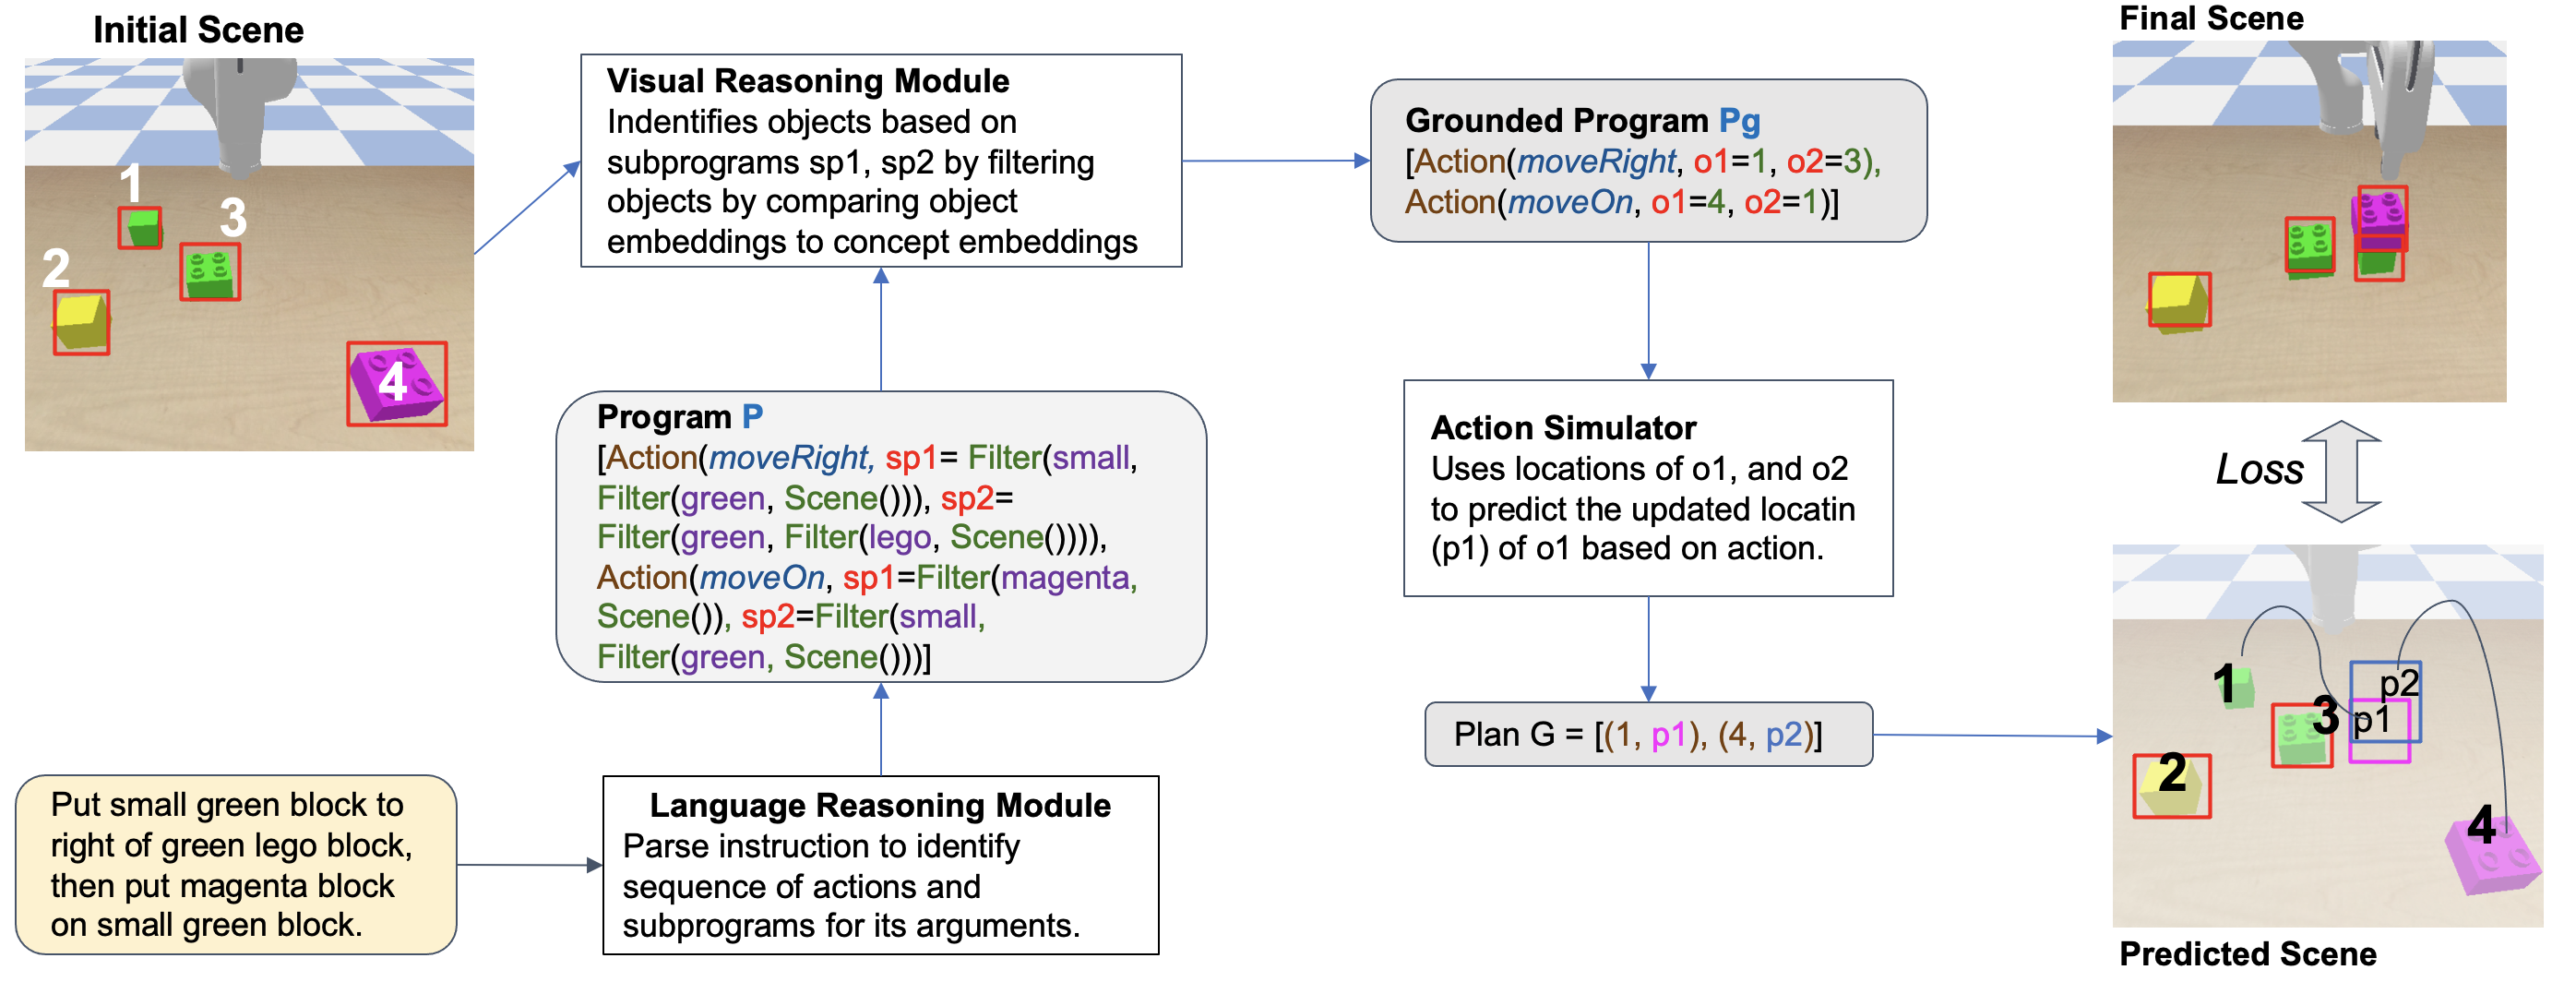
\includegraphics[width=15cm]{figures/schematic.png}
    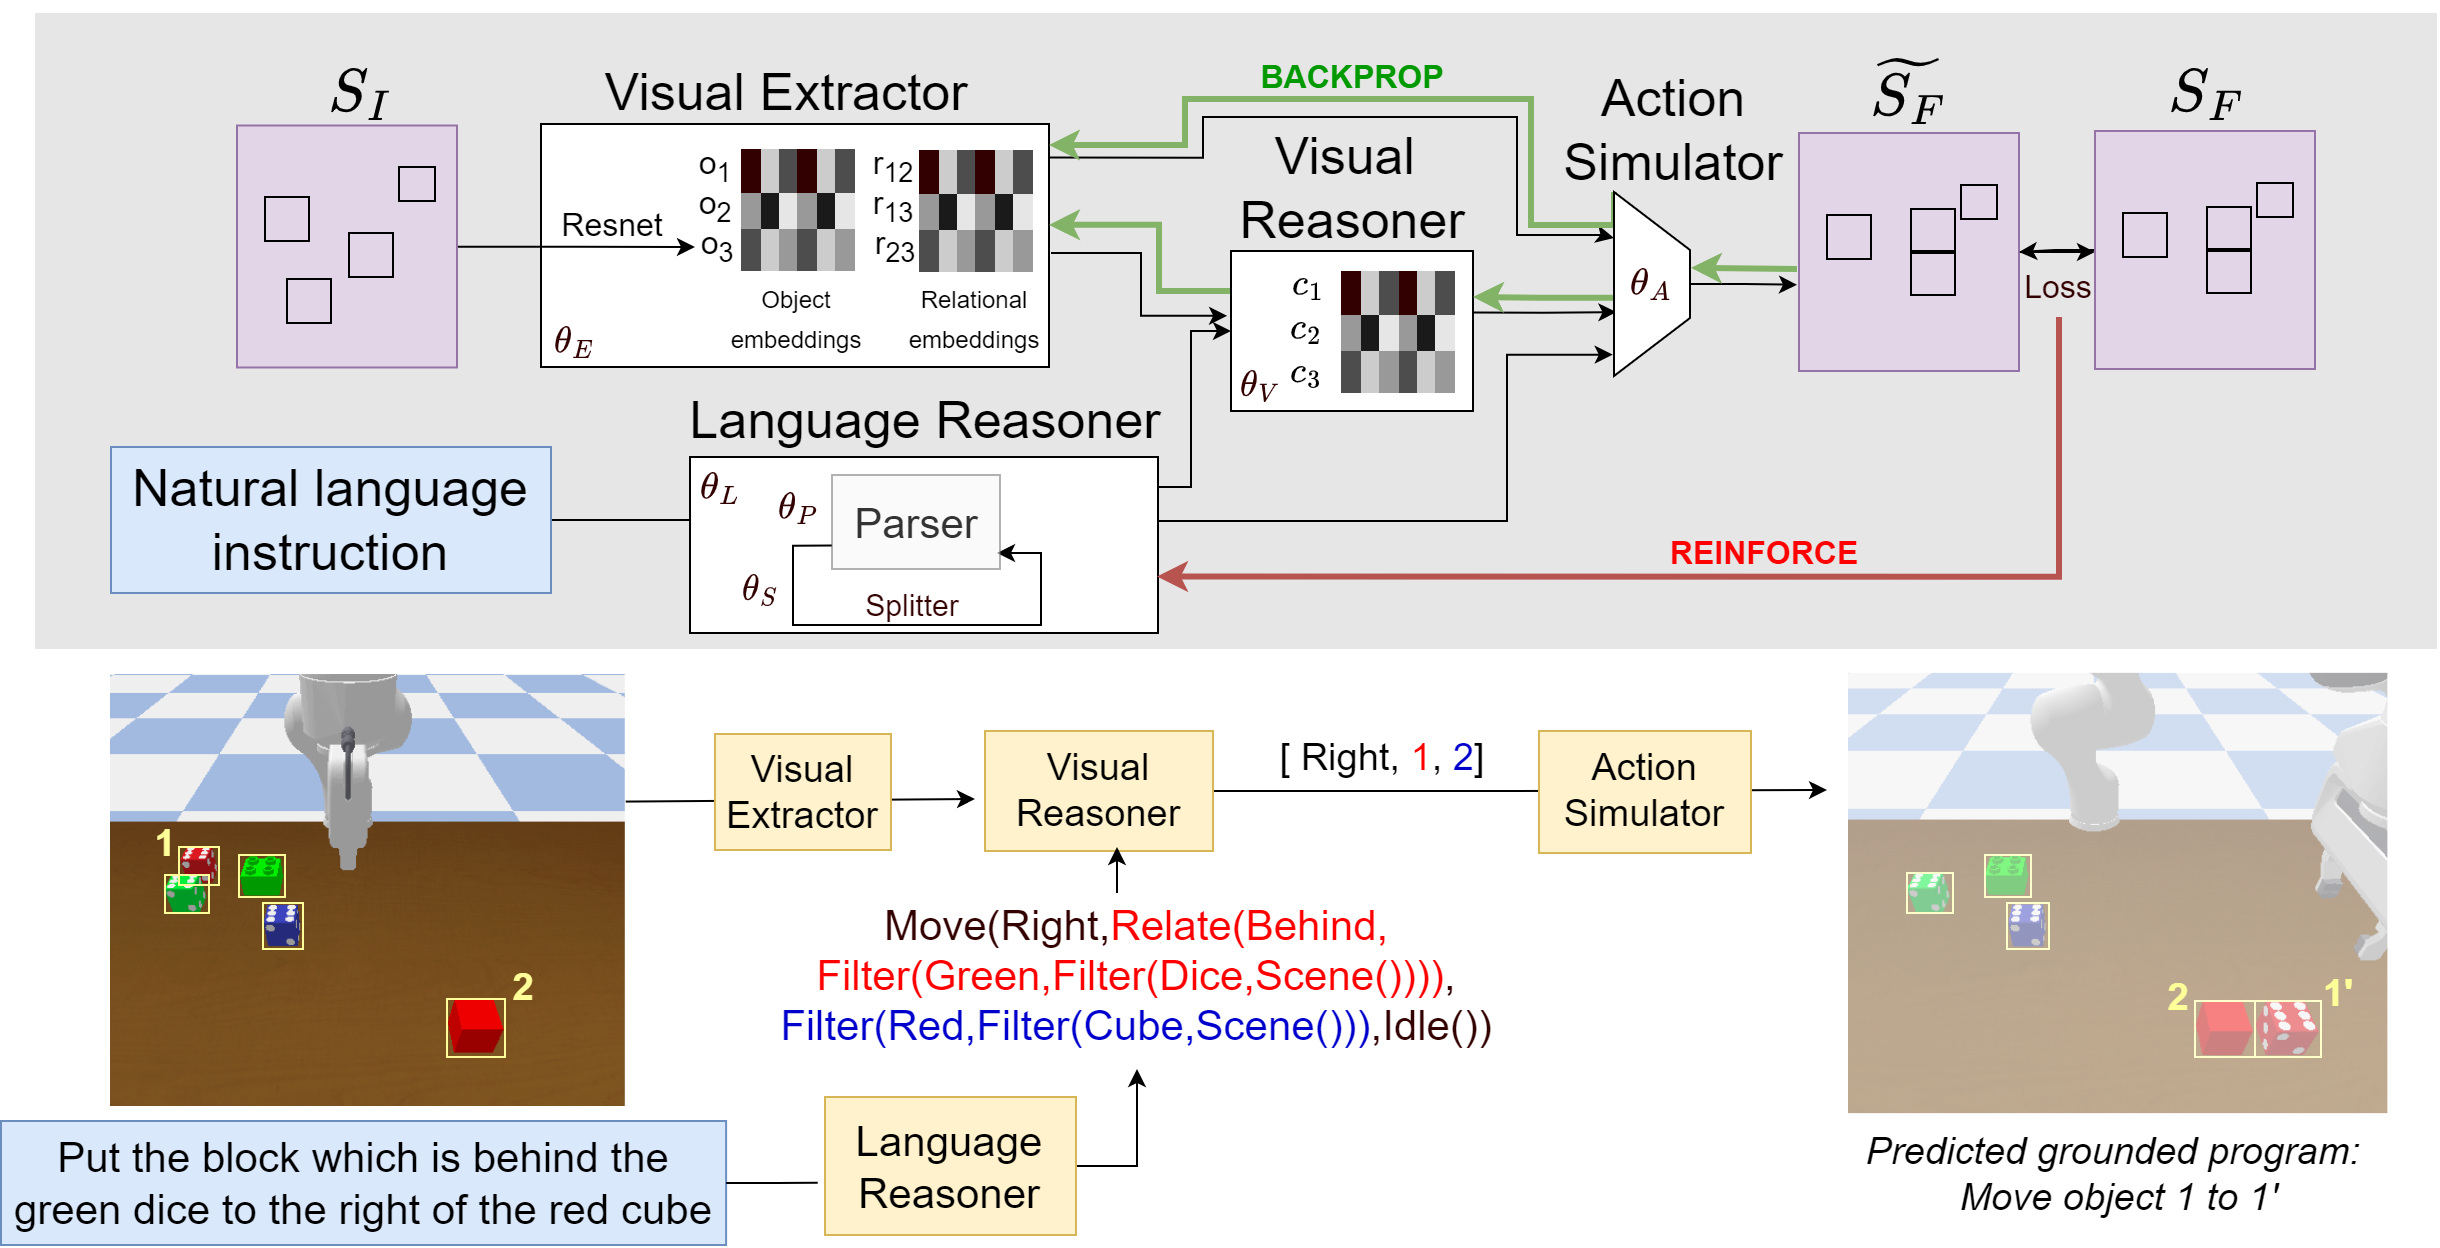
\includegraphics[width=16cm]{figures/main-model-3.png}
    
    \caption{
    \footnotesize{
    \textbf{Model architecture.} 
    %
    The \emph{Visual Extractor} forms dense object representations from the scene image using pre-trained object detector and feature extractor.  
    %
    The \emph{Language Reasoner} auto-regressively induces a symbolic program  from the instruction that represents rich symbolic reasoning over spatial and action constructs inherent in the instruction.  
    %
    The \emph{Visual Reasoner} determines which objects are affected by actions in the plan using symbolic and spatial reasoning.  
    %
    The \emph{Action Simulator} predicts final location of the moved object. 
    %
    The model is trained end-to-end with a loss on the bounding boxes, 
    %Training loss is computed between between object positions predicted by the program and those in the ground truth final scene. 
    %
    backpropagated to action and visual modules. REINFORCE is used to train \cite{williams1987class} the language reasoner from which symbolic programs are sampled.     }
    \vspace{-0.5cm}}
    
    % \caption{
    % \footnotesize{
    % The figure illustrates the inference and execution 
    % of a neuro-symbolic program for the instruction, 
    % \emph{``put the small green block to the right of the green lego block and then put the magenta block on the small green block"} provided to a robot manipulator. 
    % %
    % The natural language instruction is input to the Language Reasoning Module, which outputs a Program (P), i.e., a sequence of parsed instructions. 
    % %
    % This program P, along with the visual scene ($S_I$) is passed to the Visual Reasoning Module, which filters relevant objects from the scene, and uses them to the output a grounded program $P_g$ in which filter commands have been replaced by specific object references. 
    % %
    % The Action Simulator takes the action identifier (from the parser), locations of object arguments as output by visual reasoner, and produces resulting location of argument 1 object of the action command. It also results in outputting of sub-goals ($o,p$), which is pair of object and position combination denoting that object $o$ has to be moved to position $p$ during actual robot execution. During training, loss is back-propagated by comparing the location (bounding box) of each object in the final scene with those predicted by the model.}}
    \label{fig:schematic}
\end{figure*}









%%%% ATTIC %%%
\iffalse
\section{Introduction}
\label{sec:intro}
As robots enter human-centric environments they must be endowed the ability to 
learn to act and achieve the intended goal based on natural language instructions 
from a human partner. 
%
We consider the problem of learning to translate high level language instructions into 
executable symbolic programs grounded in the robot’s state and action space. 
%
This work focuses on  
manipulation tasks that involve complex object interactions (stacking, assembly and 
positioning in relation to other objects) executed over multiple (2-5) time steps. 
%
For example, consider instructing a manipulator to ``put the small green block to the right of the green lego block and then put the magenta block on the small green block" (see Figure 1). 
%
We assume the presence of natural supervision from a human teacher in the form of 
state transitions and linguistic description for a high-level task and aim to 
acquire a semantic representation for actions amenable to strong 
compositional generalization to novel tasks unseen during training.  
%
This learning tasks is challenging due to: (i) grounded actions have to be parsed from the underlying sentence requiring complex natural language reasoning and (ii) the affect of executing these actions has to be deciphered on the underlying scene, again requiring complex reasoning now at the image level. Further, if the supervision is provided as an image of the final scene, the model must learn a representation for intermediate actions to be executed for achieving the desired affect.

%
Present approaches fall in two categories. Pure neural-imitation 
approaches lean a direct mapping from task instructions to low-level motions and have been successful in learning motion skills or primitives like sliding, moving to a goal etc. However, such approaches are less generalizable to longer horizon manipulation tasks involving object interactions. Efforts such as ~\cite{paxton2019prospection} make progress towards learning sub-goal sequences corresponding to a high-level instructions. However, the decoded actions possess 
syntactic labels and lack a deep grounded semantics and hence less amenable to symbolic reasoning and execution.  
%
Other approaches \cite{shah2018bayesian} assume a formal representations such as LTL that is amenable 
to reasoning and verification and focus on learn a mapping from language to a symbolic representation and delegate the grounding of symbols to separate process. 

%
\textbf{Contributions.} 
This paper presents a neuro-symbolic approach for jointly learning grounded action concepts that can be composed in manipulation programs that explains how the world scene is likely to affected by the input instruction. 
%We build on the current state-of-the-art, and propose a model for grounding of concepts in a natural language instruction, to those present in the image, and translate them into actions specified as part of an executable program. 
Our action representation is purely neural, and our model results in a disentangled representation for actions.  The output of our model is a program, which when executed by the robot, results in the desired world state. Our model is trained end-to-end without any intermediate supervision. 
In summary, we make the following contributions:  
(i) a neuro-symbolic model that learns to perform object manipulation tasks requiring reasoning over scenes from the natural language instruction, and initial and final image
(ii) learning dense representations for robot manipulation actions;
(iii) learning tasks through an intermediate execution program that makes the model interpretable.
(iv) a novel loss function and a selection mechanism for actions based on gumble soft-max.
(v) instruction following experiments with a 7-dof Franka Emika robot manipulator demonstrating compositional generalization in a simulated workspace. The code and data set is available at \url{https://github.com/dair-iitd/nsrmp}.  

%online.\footnote{\url{https://github.com/dair-iitd/nsrmp}} 

\begin{figure*}
    \centering    
    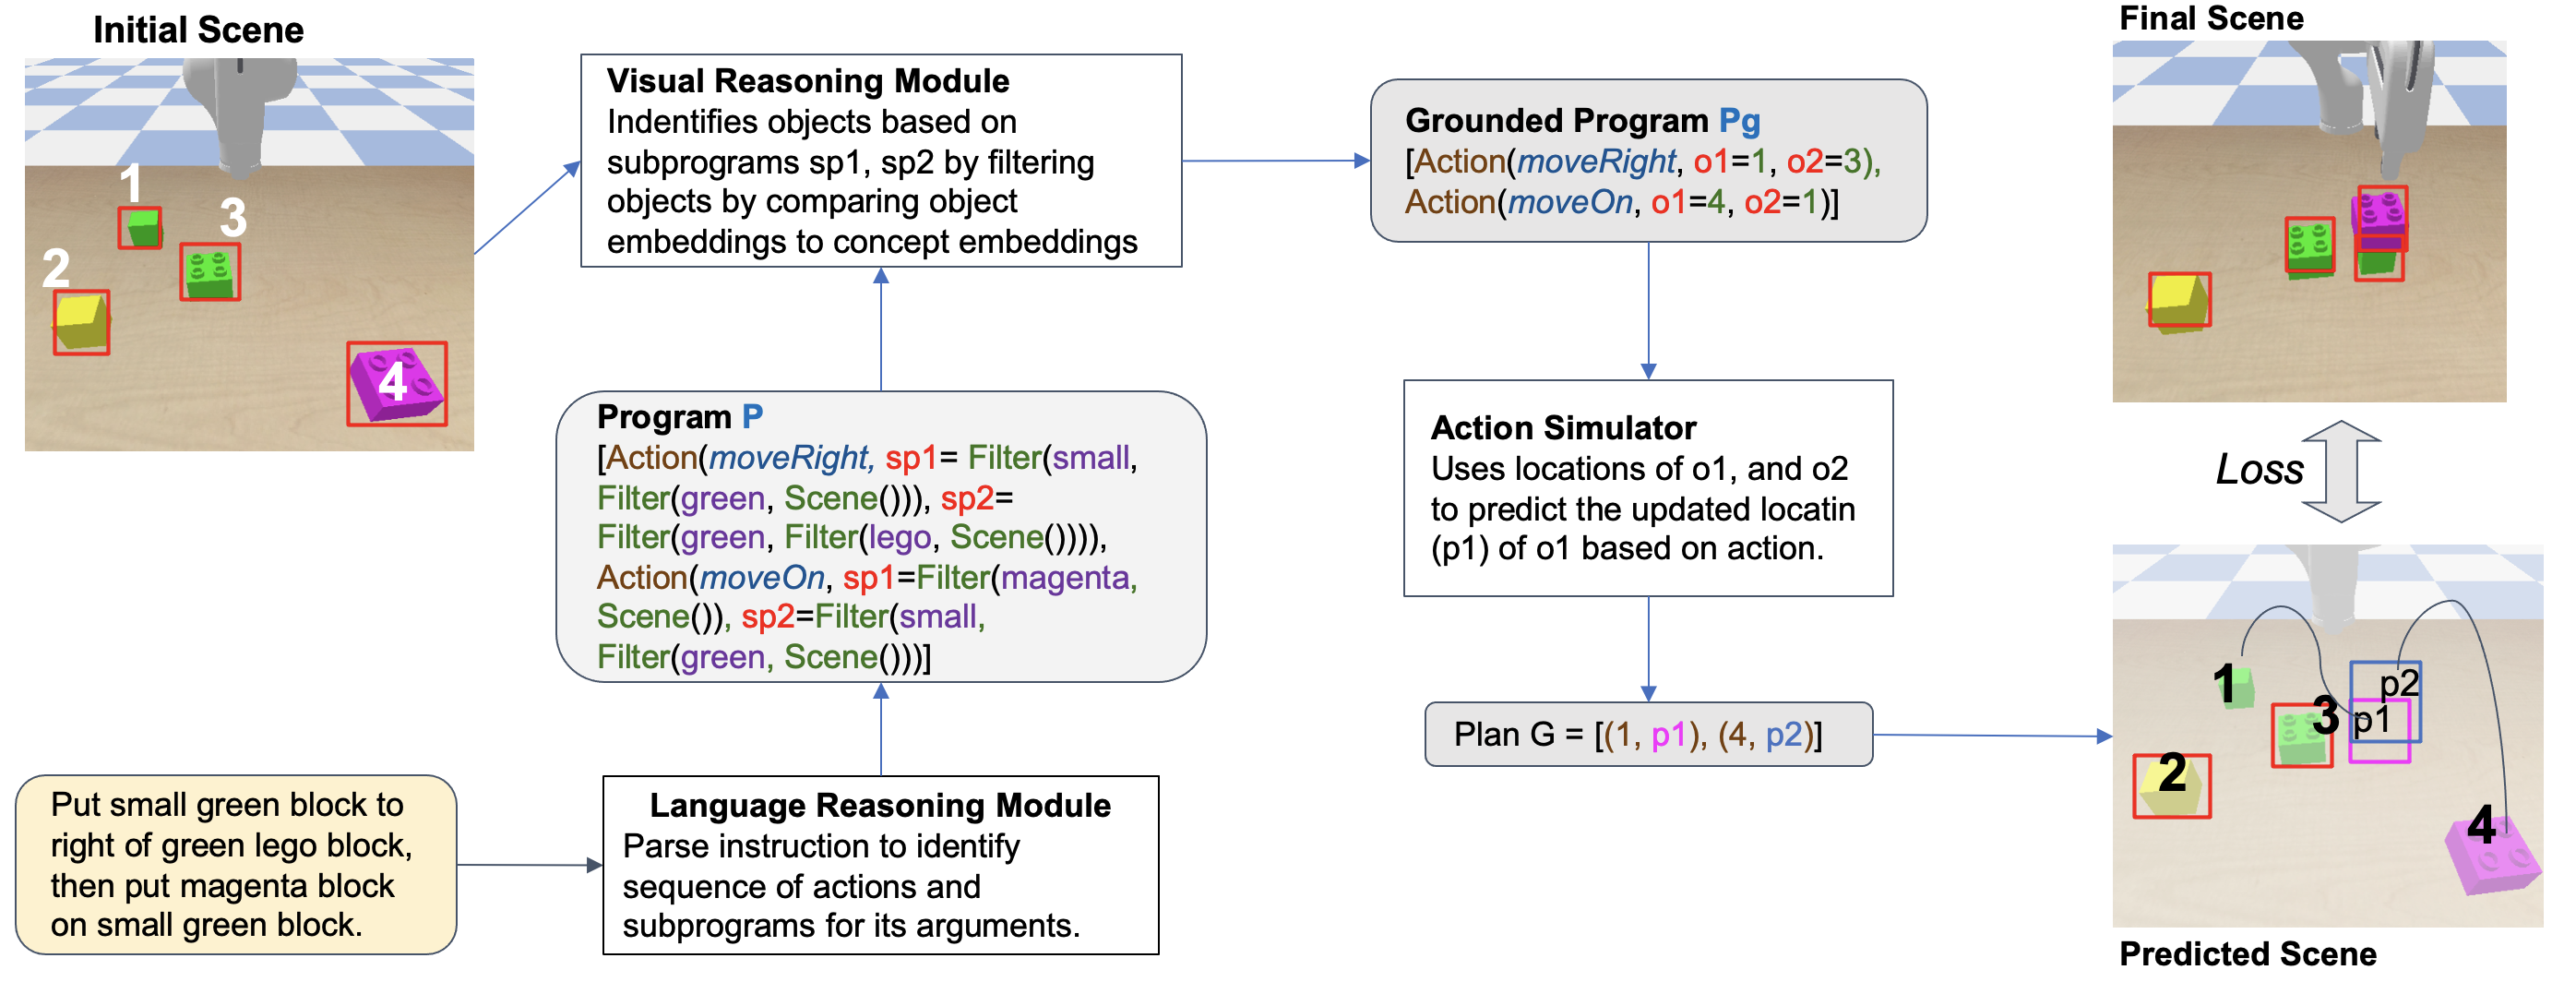
\includegraphics[width=15cm]{figures/schematic.png}
    \caption{
    \footnotesize{
    The figure illustrates the inference and execution 
    of a neuro-symbolic program for the instruction, 
    \emph{``put the small green block to the right of the green lego block and then put the magenta block on the small green block"} provided to a robot manipulator. 
    %
    The natural language instruction is input to the Language Reasoning Module, which outputs a Program (P), i.e., a sequence of parsed instructions. 
    %
    This program P, along with the visual scene ($S_I$) is passed to the Visual Reasoning Module, which filters relevant objects from the scene, and uses them to the output a grounded program $P_g$ in which filter commands have been replaced by specific object references. 
    %
    The Action Simulator takes the action identifier (from the parser), locations of object arguments as output by visual reasoner, and produces resulting location of argument 1 object of the action command. It also results in outputting of sub-goals ($o,p$), which is pair of object and position combination denoting that object $o$ has to be moved to position $p$ during actual robot execution. During training, loss is back-propagated by comparing the location (bounding box) of each object in the final scene with those predicted by the model.}}
    \label{fig:schematic}
\end{figure*}


\fi